\documentclass{scrartcl}

\usepackage{hyperref}
\usepackage{lscape}
\usepackage{graphicx}
\usepackage{adjustbox}
\usepackage{placeins}

\author{Caitlin Halfacre}
\date{\today}
\title{NICD Data Scientist - Task A3}

\begin{document}
\maketitle
I have chosen to use a Bayesian regression model to fit the clients desire for a model that both describes more of the variance in the data than their existing model and maintains predictive accuracy. While Bayesian modelling is computationally and technically more complex than a standard linear regression model, the approach to prediction and inference is more intuitive, that is, in line with how the human brain processes probability, and enables the option to present percentage likelihoods in explanations of valuations. In my analysis of the model I present visualisations and phrasing that could be used to explain valuation decisions to clients, regulators, and internal stakeholders.

\FloatBarrier
\section{Model Design}
\subsection{Priors}
The priors are set using a  weakly informative understanding of the average and maximum likely values for the data\footnote{for example, \url{https://www.chroniclelive.co.uk/news/north-east-news/most-expensive-north-east-houses-30988236} the most expensive house sold in the North East in 2024}. As discussed in section \ref{limitations} these can be improved with greater research of the property market and discussion with the client.

\subsection{Model Selection}
Model selection was performed bby building all possible models with the given predictors and comparing them using Leave One Out cross-validation, which compares predictive performance. The best model includes all available predictors and describes 76.3\% of the variance.

\FloatBarrier
\section{Model Analysis}
\begin{landscape}
	\begin{table}[htbp]
		\centering
		\caption{Regression Coefficients of the final model, including conversion from log values} 
		\label{tab:regcoef}
		\begin{adjustbox}{max width=\linewidth}
		\begin{tabular}{llllrrrrrrr}
			\hline
			effect & component & group & term & estimate & std.error & conf.low & conf.high & conv\_estimate & conv\_conf.low & conv\_conf.high \\ 
			\hline
			fixed & cond &  & (Intercept) & 10.53 & 0.09 & 10.36 & 10.70 & 37382.52 & 31556.14 & 44413.54 \\ 
			fixed & cond &  & locationGateshead & 0.93 & 0.06 & 0.81 & 1.06 & 95139.57 & 84248.10 & 107610.30 \\ 
			fixed & cond &  & locationMorpeth & 0.40 & 0.07 & 0.26 & 0.54 & 55559.25 & 48488.83 & 63871.28 \\ 
			fixed & cond &  & locationNewcastle & 1.22 & 0.06 & 1.10 & 1.34 & 126393.23 & 112033.94 & 142423.59 \\ 
			fixed & cond &  & locationSunderland & 0.36 & 0.07 & 0.23 & 0.49 & 53720.81 & 47109.97 & 61286.62 \\ 
			fixed & cond &  & bedrooms & 0.04 & 0.01 & 0.02 & 0.06 & 38794.91 & 38051.78 & 39587.98 \\ 
			fixed & cond &  & bathrooms & 0.10 & 0.03 & 0.04 & 0.15 & 41221.60 & 39057.39 & 43535.46 \\ 
			fixed & cond &  & size\_sqft & 0.00 & 0.00 & 0.00 & 0.00 & 37409.69 & 37407.29 & 37412.14 \\ 
			fixed & cond &  & ownershipFreehold & -0.03 & 0.03 & -0.09 & 0.03 & 36195.52 & 33999.73 & 38482.48 \\ 
			fixed & cond &  & ownershipLeasehold & -0.06 & 0.03 & -0.12 & 0.00 & 35217.19 & 33050.49 & 37522.71 \\ 
			fixed & cond &  & ownershipUnknown & -0.05 & 0.04 & -0.13 & 0.03 & 35558.43 & 32923.32 & 38414.76 \\ 
			fixed & cond &  & property\_typeDetached & -0.01 & 0.05 & -0.10 & 0.09 & 37149.24 & 33830.07 & 40771.30 \\ 
			fixed & cond &  & property\_typeFlat & -0.02 & 0.05 & -0.11 & 0.07 & 36774.88 & 33605.19 & 40236.22 \\ 
			fixed & cond &  & property\_typeMansionette & -0.01 & 0.05 & -0.11 & 0.09 & 37036.55 & 33418.08 & 41037.50 \\ 
			fixed & cond &  & property\_typeNotSpecified & -0.02 & 0.05 & -0.12 & 0.08 & 36676.94 & 33279.02 & 40356.21 \\ 
			fixed & cond &  & property\_typeSemiMDetached & -0.01 & 0.04 & -0.09 & 0.07 & 37088.74 & 34145.29 & 40240.16 \\ 
			fixed & cond &  & property\_typeTerraced & 0.01 & 0.04 & -0.08 & 0.09 & 37645.75 & 34526.57 & 40938.13 \\ 
			fixed & cond &  & gardenNotSpecified & 0.05 & 0.03 & -0.01 & 0.12 & 39387.55 & 36929.86 & 42024.05 \\ 
			fixed & cond &  & gardenPatio & 0.03 & 0.05 & -0.07 & 0.12 & 38423.84 & 34964.36 & 41971.31 \\ 
			fixed & cond &  & gardenYes & 0.00 & 0.02 & -0.04 & 0.05 & 37435.81 & 35785.83 & 39150.95 \\ 
			ran\_pars & cond & Residual & sd\_\_Observation & 0.27 & 0.01 & 0.25 & 0.28 & 48826.68 & 48220.18 & 49480.30 \\ 
			\hline
		\end{tabular}
	\end{adjustbox}
	\end{table}
\end{landscape}


Table \ref*{tab:regcoef} is a full summary of the model including conversions from the log values. To demonstrate the predictions table \ref{tab:pred} is predicted prices for ten random properties. It can be stated that the mean likely value is as in the prediction column andthere is a 67\% likelihood that the price will be between the values in columns Q16.5 and Q83.5. Any future property can be predicted in the same way.

\begin{landscape}
	% latex table generated in R 4.4.1 by xtable 1.8-4 package
	% Mon Aug  4 00:30:04 2025
	\begin{table}[htbp]
		\centering
		\caption{Example predictions} 
		\label{tab:pred}
		\begin{adjustbox}{max width=\linewidth}
		\begin{tabular}{lrrrlllrrrr}
			\hline
			location & bedrooms & bathrooms & size\_sqft & ownership & property\_type & garden & prediction & Est.Error & Q16.5 & Q83.5 \\ 
			\hline
			Morpeth &   5 &   0 & 1238.00 & Unknown & Flat & Yes & 159641.20 & 45549.44 & 117288.77 & 201473.15 \\ 
			Morpeth &   5 &   1 & 2078.00 & Leasehold & Apartment & Patio & 339139.06 & 96988.67 & 249202.89 & 427569.83 \\ 
			Morpeth &   1 &   1 & 2658.00 & Unknown & Flat & Not Specified & 447402.86 & 127774.50 & 327172.25 & 565927.92 \\ 
			Consett &   4 &   1 & 828.00 & Leasehold &  & Patio & 88299.01 & 25214.50 & 64227.39 & 112093.00 \\ 
			Gateshead &   4 &   1 & 2618.00 & Unknown & Semi-Detached & No & 795624.06 & 227276.15 & 582865.16 & 1003123.13 \\ 
			Morpeth &   6 &   2 & 1298.00 & Freehold &  & No & 218279.11 & 61535.25 & 160598.80 & 273408.13 \\ 
			Newcastle &   2 &   0 & 2698.00 & Unknown & Not Specified & Patio & 965347.52 & 278475.37 & 704531.97 & 1229834.70 \\ 
			Morpeth &   5 &   1 & 2138.00 & Unknown & Not Specified &  & 338236.45 & 97544.98 & 248275.74 & 425726.72 \\ 
			Sunderland &   4 &   1 & 448.00 &  & Apartment & Yes & 98542.27 & 27582.19 & 73011.07 & 123859.88 \\ 
			Gateshead &   1 &   1 & 2798.00 & Unknown & Flat & No & 802233.74 & 230548.96 & 584704.71 & 1008796.64 \\ 
			\hline
		\end{tabular}
	\end{adjustbox}
	\end{table}

\end{landscape}

Figures \ref{fig:estimates} shows a comparison of the relative impact of the different factors on the intercept of the model. We can see from this that despite the best model including all the predictors location has the largest effect. Figures \ref{fig:celocation} and \ref{fig:cegarden} show predicted values for each of the locations and each of the garden types respectively, these show how much more variation there is between the locations than between the garden types.


\begin{figure}[htbp]
	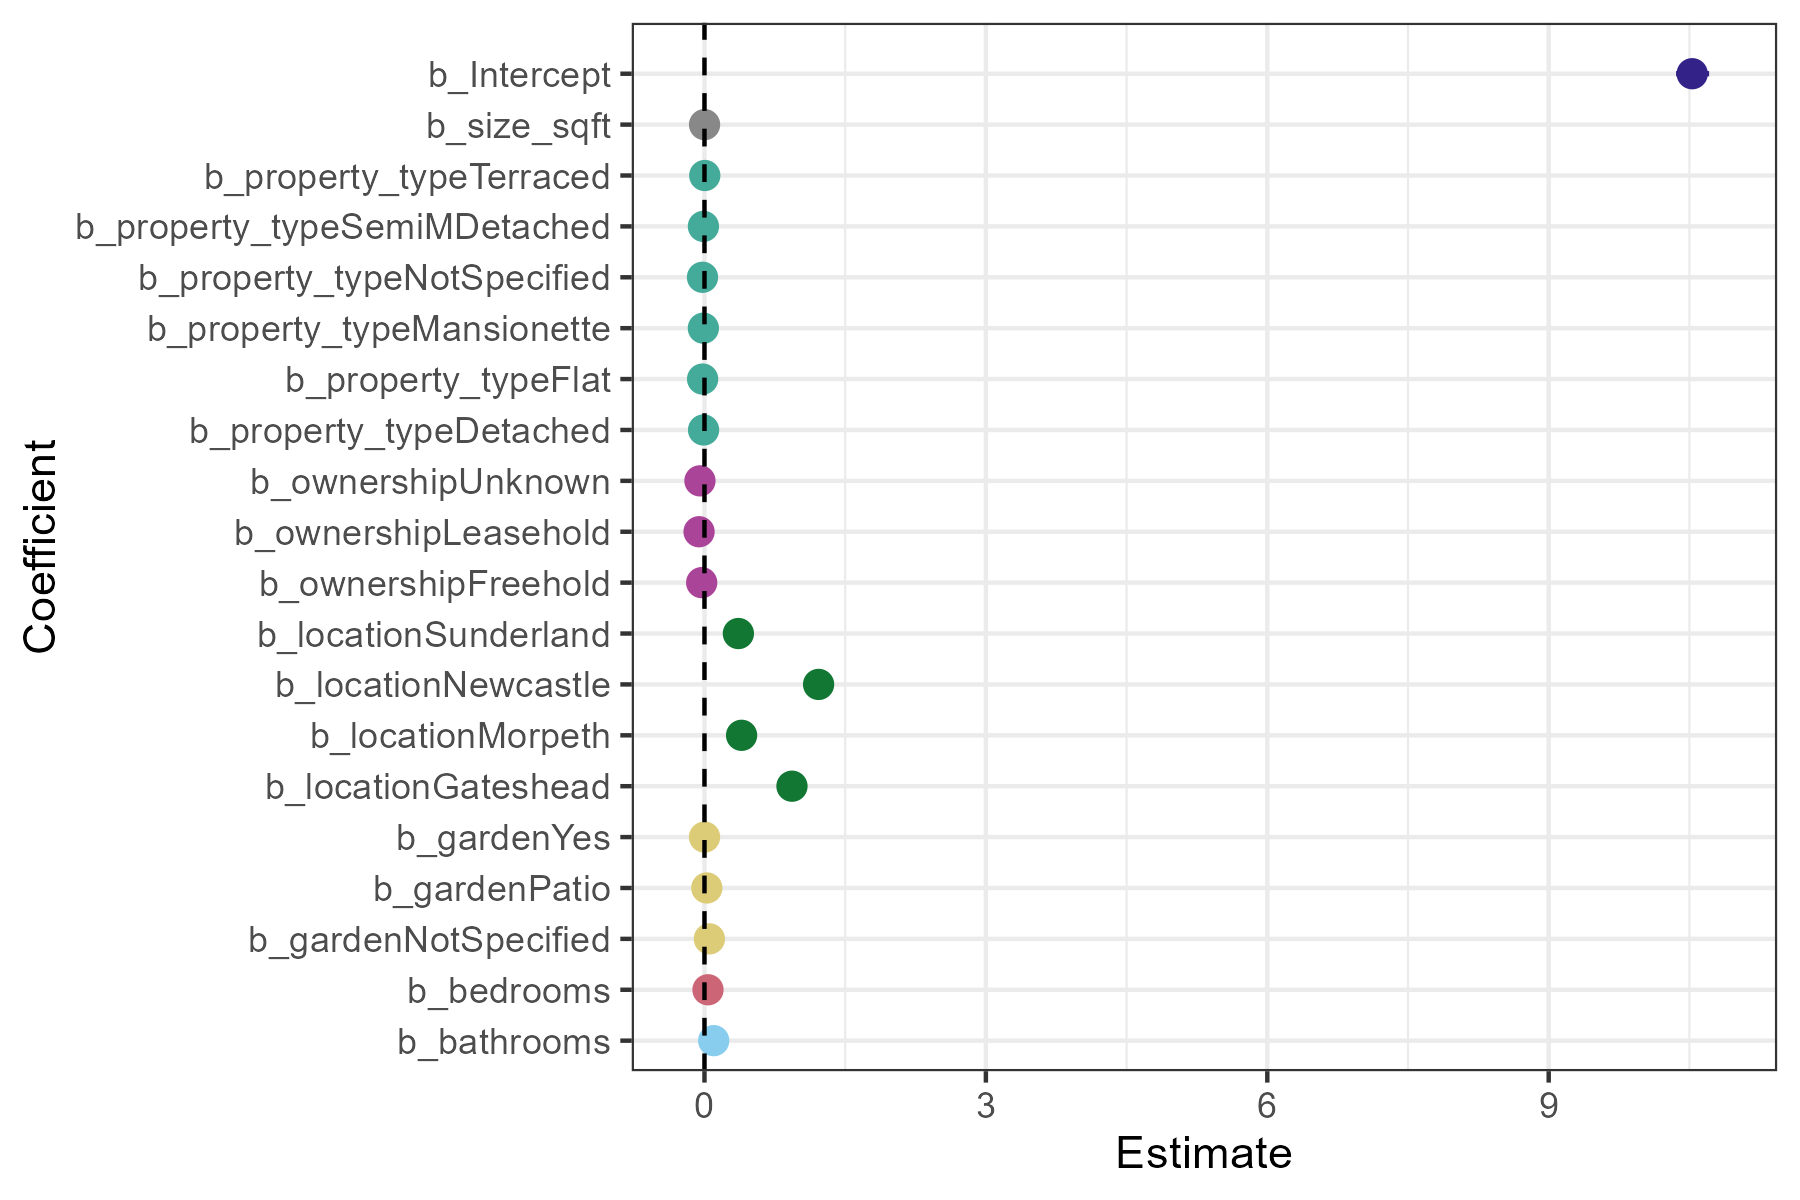
\includegraphics[width = \textwidth]{../figures/estimates.png}
	\label{fig:estimates}
	\caption{Estimates of the fitted model}
\end{figure}

\begin{figure}[htbp]
	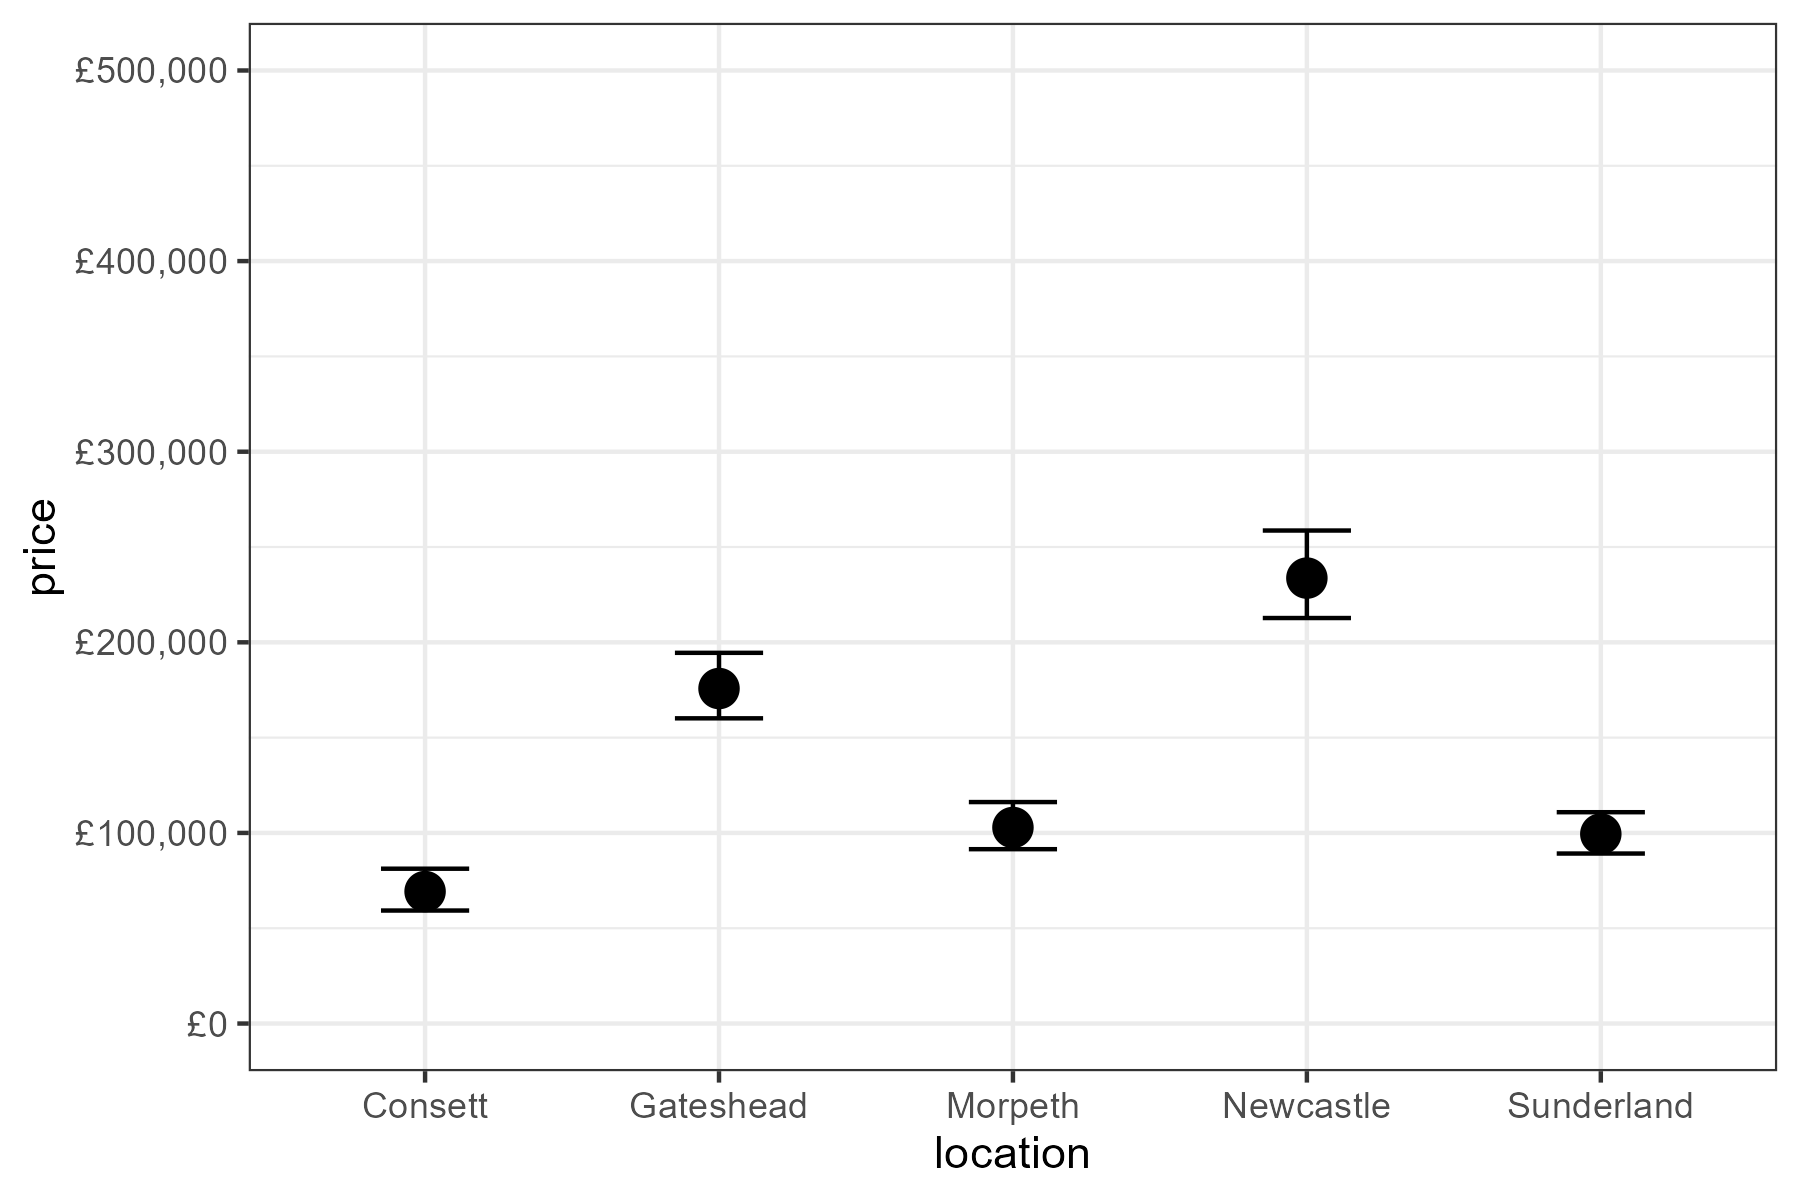
\includegraphics[width = \textwidth]{../figures/celocation.png}
	\label{fig:celocation}
	\caption{Predicted values by location}
\end{figure}

\begin{figure}[htbp]
	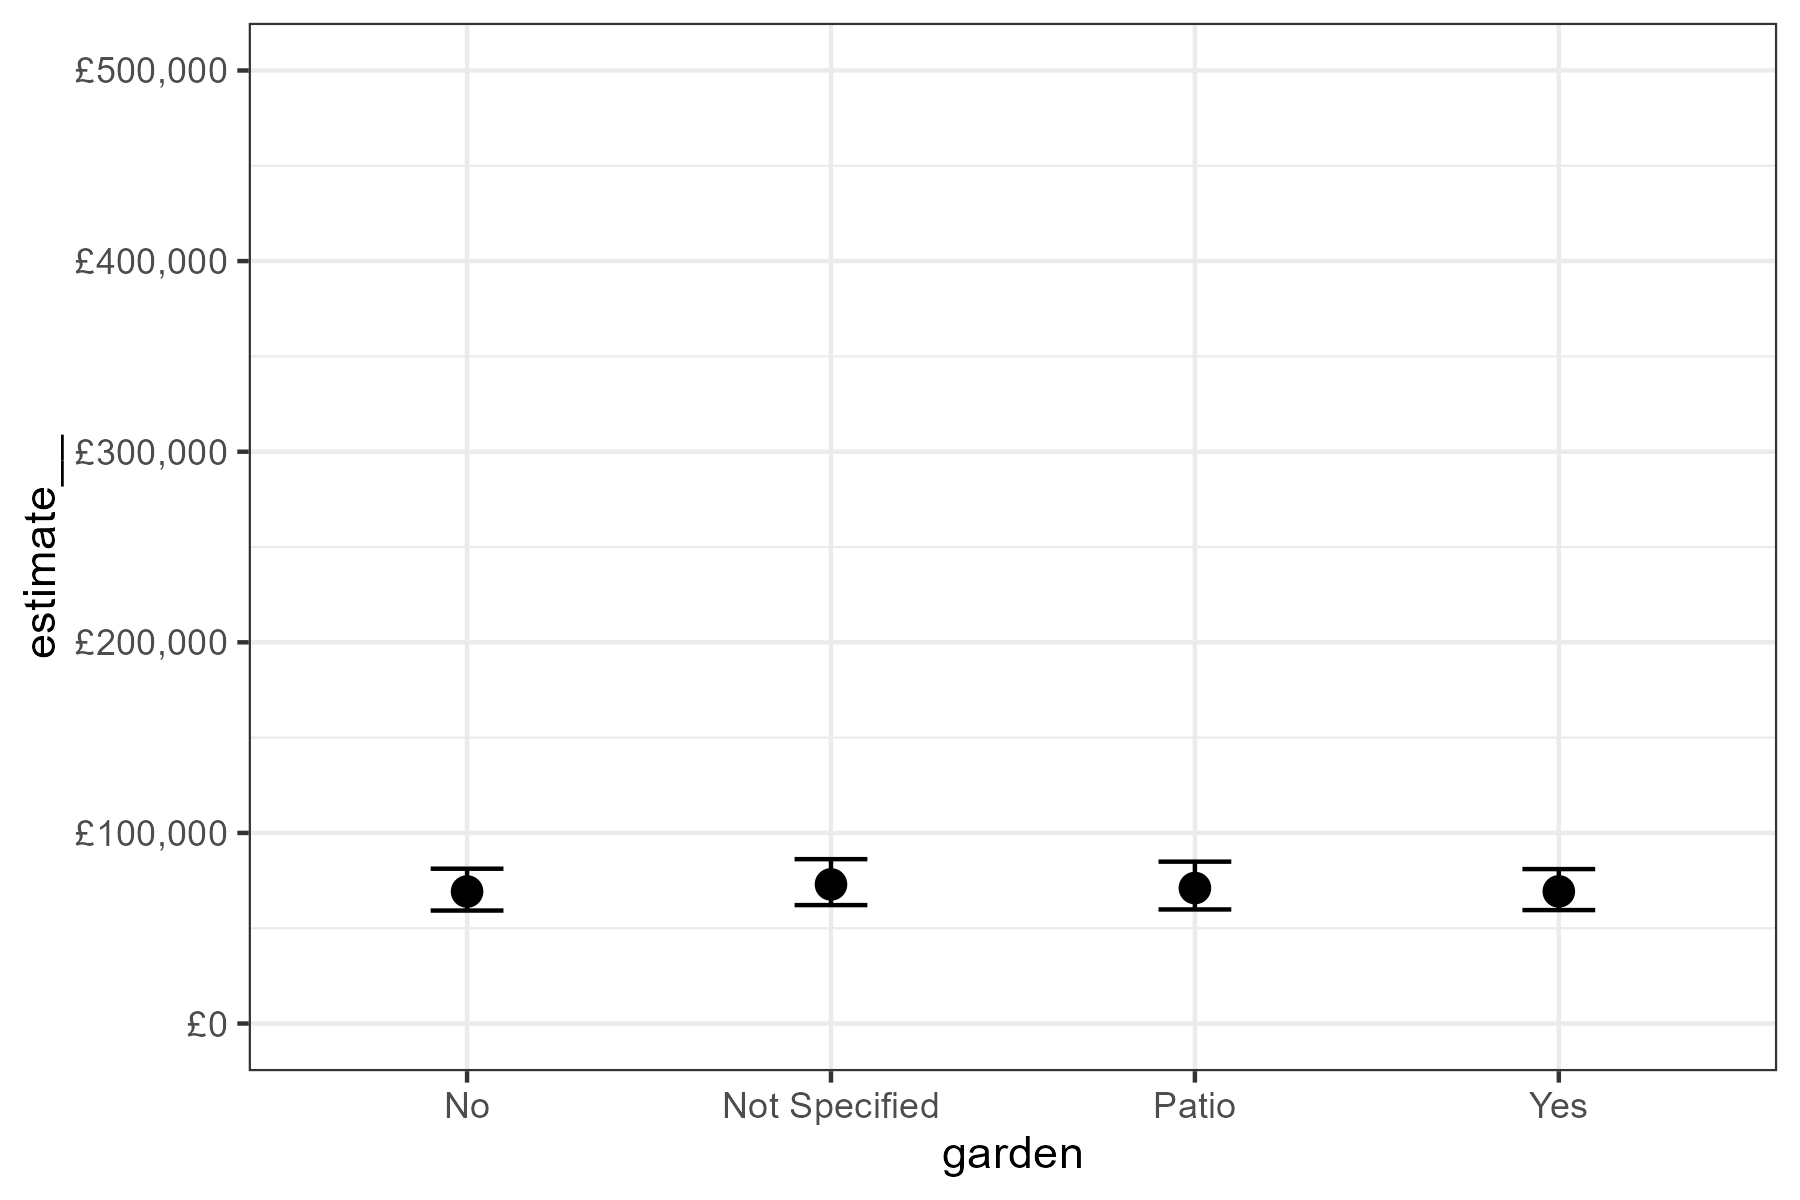
\includegraphics[width = \textwidth]{../figures/cegarden.png}
	\label{fig:cegarden}
	\caption{Predicted values by garden}
\end{figure}


\FloatBarrier
\section{Limitations and improvements} \label{limitations}
The data has some major outliers, particularly in Newcastle and Gateshead, removing this could improve the predictive power of the model. Similarly the variation between the regions is so high that in further work I would consider building separate models for each region to enable more specific predictions

One of the biggest advantages of Bayesian modelling is the ability to constrain a model using domain specific knowledge. This can be as little as knowing that a price cannot be negative, but is far more useful if more information can be added. Discussion with the client regarding for example setting the maximum likely price of a property.

There is quite a lot of unclear categorisations in the data. For example, in garden "Not Specified" and NA may be the same so could be conflated, and for property type the difference between Flat and Apartment is unclear. Seeking clarification from the client on these distinctions made could improve the predictive power of the model. 


\end{document}